\section{Método de solución}

Consideraremos una estructura de \(n\) pisos, la cual se puede modelar mediante \eqref{eqn:final-matrix-form}. Además, consideraremos que la estructura parte del reposo y de la posición de equilibrio. Esto nos aporta las condiciones iniciales \(\mathbf{u}(0) = \mathbf{0}\) y \(\mathbf{u}'(0) = \mathbf{0}\).

\subsection{Intento mediante eigenvalores y eigenvectores}

Podemos considerar el problema reducido de las ecuaciones para una estructura de \(n = 2\) pisos bajo los siguientes parámetros simplificados:
\begin{gather}
	m_1 = m_2 = m \\
	c_2 = 0, \, c_1 = c \\
	k_1 = k_2 = k \\
	P_1(t) = A\sin(\omega t), \, P_2(t) = 0
.\end{gather}

La ecuación sería la siguiente:
\[
	\begin{bmatrix}
    	m & 0 \\
    	0 & m
	\end{bmatrix} \begin{bmatrix} u_1'' \\ u_2'' \end{bmatrix}
	+ \begin{bmatrix}
    	c & 0 \\
    	0 & 0
	\end{bmatrix} \begin{bmatrix} u_1' \\ u_2' \end{bmatrix}
	+ \begin{bmatrix}
    	2k & -k \\
    	-k & k
	\end{bmatrix} \begin{bmatrix} u_1 \\ u_2 \end{bmatrix}
	= \begin{bmatrix} A\sin(\omega t) \\ 0 \end{bmatrix}
,\]

la cual se puede expresar como el sistema
\[
	\begin{cases}
    	mu_1'' + cu_1' + 2ku_1 - ku_2 = A\sin(\omega t) \\
    	mu_2'' - ku_1 + ku_2 = 0
	.\end{cases}
\]

Empezamos realizando un cambio de variable para poder construir un sistema de primer orden:
\[
	\begin{cases}
    	u_1'=v_1 \\
    	u_2'=v_2.
	\end{cases}
\]

El nuevo sistema toma la siguiente forma:
\[
	\begin{cases}
    	u_1'=v_1 \\
    	u_2'=v_2 \\
    	mv_1' + cv_1 + 2ku_1 - ku_2 = A\sin(\omega t) \\ mv_2' - ku_1 + ku_2 = 0. \end{cases}
\]

Despejado las derivadas a un lado de la ecuación, obtenemos
\[
	\begin{cases}
    	u_1' = v_1 \\
    	u_2' = v_2 \\
    	v_1' = - \frac{2k}{m}u_1 + \frac{k}{m}u_2 - \frac{c}{m}v_1 + \frac{A}{m}\sin(\omega t) \\
    	v_2' = \frac{k}{m}u_1 - \frac{k}{m}u_2.
	\end{cases}
.\]

Expresando el sistema en su forma matricial \(X' = AX\) se obtiene la expresión
\[
    \begin{bmatrix} u_1' \\ u_2' \\ v_1' \\ v_2' \end{bmatrix} =
    \begin{bmatrix}
        0 & 0 & 1 & 0 \\
   	0 & 0 & 0 & 1 \\
    -\frac{2k}{m} & \frac{k}{m} & -\frac{c}{m} & 0 \\
    \frac{k}{m} & -\frac{k}{m} & 0 & 0
    \end{bmatrix} \begin{bmatrix} u_1 \\ u_2 \\ v_1 \\ v_2 \end{bmatrix}
    + \begin{bmatrix} 0 \\ 0 \\ \frac{A}{m}\sin(\omega t) \\ 0 \end{bmatrix}
.\]

Para resolver el sistema lineal, podemos usar el método de eigenvalores y eigenvectores. Para esto, primero resolvemos el sistema homogéneo. Empezamos hallando los eigenvalores mediante la ecuación característica \(\det(A-\lambda I) = 0\):
\[
	p(\lambda ) = \begin{vmatrix}
        -\lambda & 0 & 1 & 0 \\
        0 & -\lambda & 0 & 1 \\
        -\frac{2k}{m} & \frac{k}{m} & -\frac{c}{m}-\lambda & 0 \\
        \frac{k}{m} & -\frac{k}{m} & 0 & -\lambda
   \end{vmatrix}
   = \lambda^4 + \frac{c}{m}\lambda^3 + \frac{3k}{m}\lambda^2 + \frac{ck}{m^2}\lambda + \frac{k^2}{m^2}
   = 0
.\]

Aunque tenemos una ecuación de grado 4, esta se puede resolver con métodos computacionales.

\subsection{Usando métodos numéricos}

Para resolver este sistema con las condiciones iniciales dadas, utilizaremos el método de Runge-Kutta de orden 4 (RK4), el cual se detalla en el marco teórico del informe. Sin embargo, para ello será necesario llevar \eqref{eqn:final-matrix-form} a la forma
\[
    \mathbf{x}' = \mathbf{f}(t, \mathbf{x})
.\]

Para ello, podemos definir \(\mathbf{v} = \mathbf{u}'\), lo cual transforma \eqref{eqn:final-matrix-form} (un sistema de \(n\) ecuaciones) en el siguiente sistema de \textit{primer orden} de \(2n\) ecuaciones:

\[
    \begin{cases}
        \mathbf{v} = \mathbf{u}' \\
        M\mathbf{v}' + C\mathbf{v} + K\mathbf{u} = \mathbf{P}(t)
    .\end{cases}
\]

Nótese que cada una de estas ecuaciones matriciales aporta \(n\) ecuaciones al sistema.

Para aplicar el método de RK4 a este sistema, lo colocaremos en la forma
\begin{equation}\label{eqn:substituted-system}
    \begin{cases}
        \mathbf{u}' = \mathbf{v} \\
        \mathbf{v}' = M^{-1}(-C\mathbf{v} - K\mathbf{u} + \mathbf{P}(t))
    .\end{cases}
\end{equation}

Nótese también que \(M^{-1}\) siempre existe (y es trivial) puesto que \(M\) es una matriz diagonal cuyos elementos en dicha diagonal son todos no-nulos:
\[
    M^{-1} = \begin{bmatrix}
        1/m_1 & 0 & \cdots & 0 \\
        0 & 1/m_2 & \cdots & 0 \\
        \vdots & \vdots & \ddots & \vdots \\
        0 & 0 & \cdots & 1/m_n
    \end{bmatrix}
.\]

Ahora podemos expresar \eqref{eqn:substituted-system} mediante una sola ecuación matricial con \(\mathbf{u}\) y \(\mathbf{v}\) concatenados en un solo vector \(\mathbf{x}\) como
\begin{equation}\label{eqn:rk4-ready}
    \mathbf{x}' = \mathbf{f}(t, \mathbf{x})
,\end{equation}
donde definimos
\[
    \mathbf{x} = \begin{bmatrix} \mathbf{u} \\ \mathbf{v} \end{bmatrix}_{2n \times 1},
    \qquad
    \mathbf{f}(t, \mathbf{x}) = \mathbf{f}\left(t, \begin{bmatrix} \mathbf{u}_{n \times 1} \\ \mathbf{v}_{n \times 1} \end{bmatrix}\right) = \begin{bmatrix}
        \mathbf{v} \\
        M^{-1}(-C\mathbf{v} - K\mathbf{u} + \mathbf{P}(t))
    \end{bmatrix}_{2n \times 1}
.\]

Nótese que las condiciones iniciales que establecimos (\(\mathbf{u}(0) = \mathbf{u}'(0) = \mathbf{v}(0) = \mathbf{0}\)) producen en conjunto la condición \(\mathbf{x}(0) = \mathbf{0}\). Además, trabajaremos RK4 con el tiempo inicial \(t_0 = 0\).

Entonces, el procedimiento que usaremos será el siguiente:

\begin{enumerate}
    \item Definir un tiempo final \(t_s\) y una cantidad \(s\) de pasos.
    \item Calcular el avance por iteración: \(h = \frac{t_s - t_0}{s}\).
    \item Comenzando en \(t_0 = 0, \mathbf{x}_0 = \mathbf{0}\), iterar \(s\) veces el método de RK4 de la siguiente manera:
        \begin{enumerate}

            \item Calcular, en orden, los siguientes vectores:
                \begin{align*}
                    \mathbf{k}_1 &= \mathbf{f}(t_i, \mathbf{x}_i) \\
                    \mathbf{k}_2 &= \mathbf{f}(t_i + \frac{h}{2}, \mathbf{x}_i + \frac{h}{2}\mathbf{k}_1) \\
                    \mathbf{k}_3 &= \mathbf{f}(t_i + \frac{h}{2}, \mathbf{x}_i + \frac{h}{2}\mathbf{k}_2) \\
                    \mathbf{k}_4 &= \mathbf{f}(t_i + h, \mathbf{x}_i + h\mathbf{k}_3)
                .\end{align*}

            \item Calcular la siguiente iteración de \(\mathbf{x}\) como
                \[
                    \mathbf{x}_{i+1} = \mathbf{x}_i + \frac{h}{6}(\mathbf{k}_1 + 2\mathbf{k}_2 + 2\mathbf{k}_3 + \mathbf{k}_4)
                \]
                y la siguiente iteración de \(t\) como \(t_{i+1} = t_i + h\).
        \end{enumerate}
\end{enumerate}

Al final del proceso, los valores de \(\mathbf{x}\) obtenidos contendrán en sus primeras mitades los puntos calculados para las posiciones \(u_1, u_2, \ldots, u_n\) de los pisos a través del tiempo.

Nótese que, en lugar de definir explícitamente un valor para el avance \(h\), definimos un \textit{tiempo final} \(t_s\) y calculamos \(h\) en función de este y la cantidad de pasos deseada, puesto que resulta más conveniente definir un tiempo de llegada y una cantidad de pasos que denoten la ``precisión'' a utilizar.

Los resultados presentados a continuación fueron obtenidos con una precisión de \(s = 10,000\) pasos.

\subsubsection*{Resultados para parámetros particulares}

Se presentan a continuación las gráficas resultantes para ciertos conjuntos de parámetros particulares. La implementación en Python de RK4 usada se encuentra en el apéndice~\ref{appendix:rk4-code}.

Los valores de masa, amortiguamiento y elasticidad que utilizaremos se basan en el trabajo de \citet{tarque}, quienes presentan los siguientes parámetros para un edificio de tres pisos de un estudio real:
\begin{gather}
    m_1 = m_2 = m_3 = 150 \, \si{ton} = 150,000 \, \si{kg}, \\
    k_1 = k_2 = k_3 = 200,000 \, \si{N/m}, \\
    \zeta_1 = 5\%, \quad \zeta_2 = \zeta_3 = 0\%
,\end{gather}
de donde (como se explicó en el marco teórico sobre las razones de amortiguamiento) tenemos los coeficientes de amortiguamiento \(c_1 = 5\%(2\sqrt{m_1 k_1}) \approx 16497.13 \, \si{kg/s}, \,
c_2 = c_3 = 0 \, \si{kg/s}\). Aunque se tratan de parámetros para un edificio, estos parámetros son de igual manera una referencia válida para parámetros de un puente de 3 pisos.

Cabe destacar que todas las gráficas usarán segundos para el tiempo \(t\) y metros para los desplazamientos \(u_1, u_2, \ldots, u_n\).

En primer lugar, podemos considerar una fuerza externa nula \(\mathbf{P}(t) = \mathbf{0}\). La figura~\ref{fig:sol-p-0} muestra que, como es de esperarse, ninguno de los pisos presenta movimiento alguno.

\begin{figure}[ht!]
    \centering
    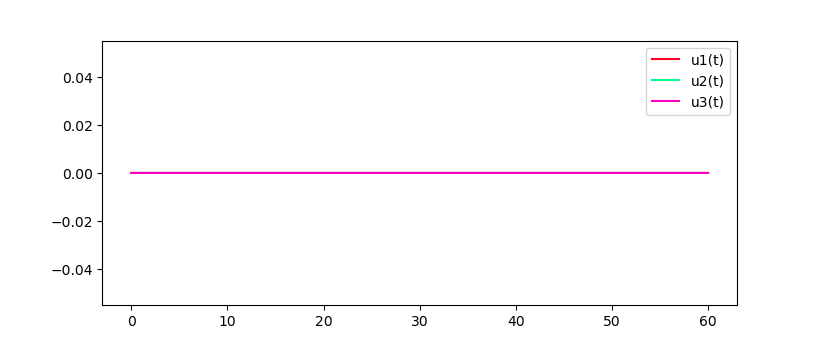
\includegraphics[width=\textwidth]{sol_p_0}
    \caption{Gráfica de \(\mathbf{u}(t)\) con \(\mathbf{P}(t) = \mathbf{0}\) para \(t \in [0, 60]\)}
    \label{fig:sol-p-0}
\end{figure}

En segundo lugar, consideramos una fuerza externa de la forma \(P_1(t) = m_1 a_g(t)\) ejercida sobre el primer piso. Esta tipo de función se utiliza para representar la fuerza ejercida sobre la base de una estructura durante un sismo \citep{kramer}, donde \(a_g(t)\) es la aceleración del suelo en función del tiempo. En particular, tomaremos \(a_g\) como una sinusoidal de la forma \(a_g(t) = A\sin(2\pi f t)\), donde \(A\) (en \(\si{m/s^2}\)) es la aceleración pico del suelo y \(f\) (en \(\si{Hz}\)) es su frecuencia de oscilación.

Tomando una aceleración pico de \(A = 0.3\) y frecuencia de oscilación de \(f = 4 \, \si{Hz}\), obtenemos la figura~\ref{fig:sol-sismo-corto}.

\begin{figure}[ht!]
    \centering
    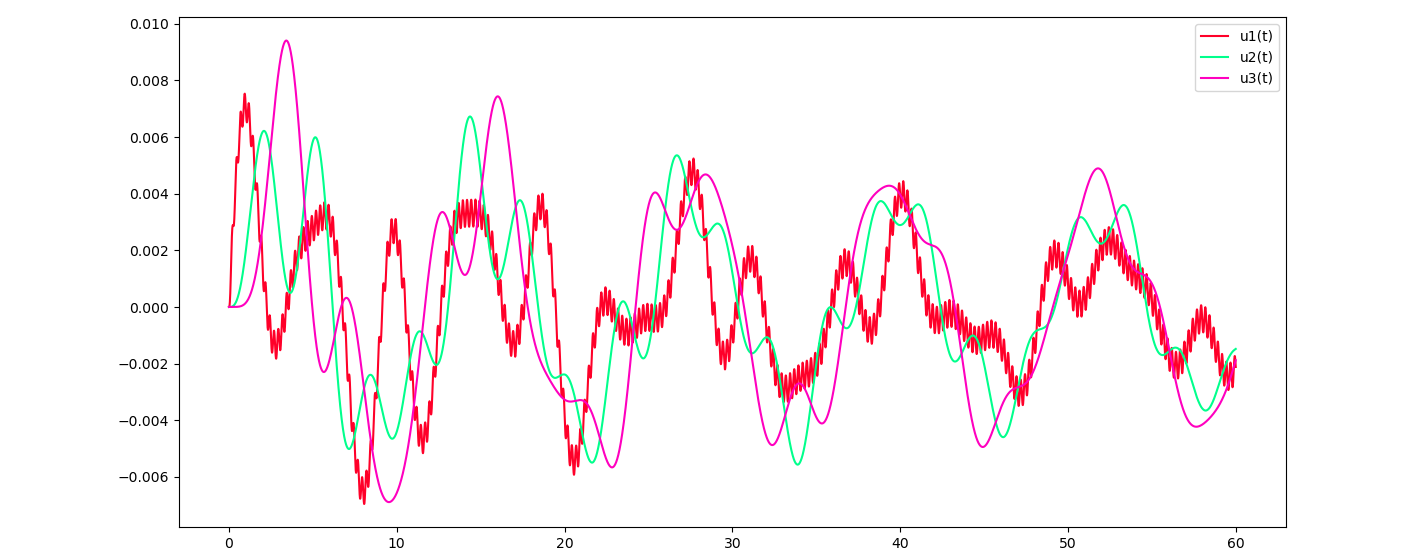
\includegraphics[width=\textwidth]{sol_sismo_corto}
    \caption{Gráfica de \(\mathbf{u}(t)\) con \(P_1(t) = m_1 A \sin(2\pi f t)\) para \(t \in [0, 60]\).}
    \label{fig:sol-sismo-corto}
\end{figure}

Sin embargo, se puede apreciar mejor el comportamiento a largo plazo de las vibraciones si extendemos la gráfica hasta un tiempo de 180 segundos (véase la figura~\ref{fig:sol-sismo-largo}).

\begin{figure}[ht!]
    \centering
    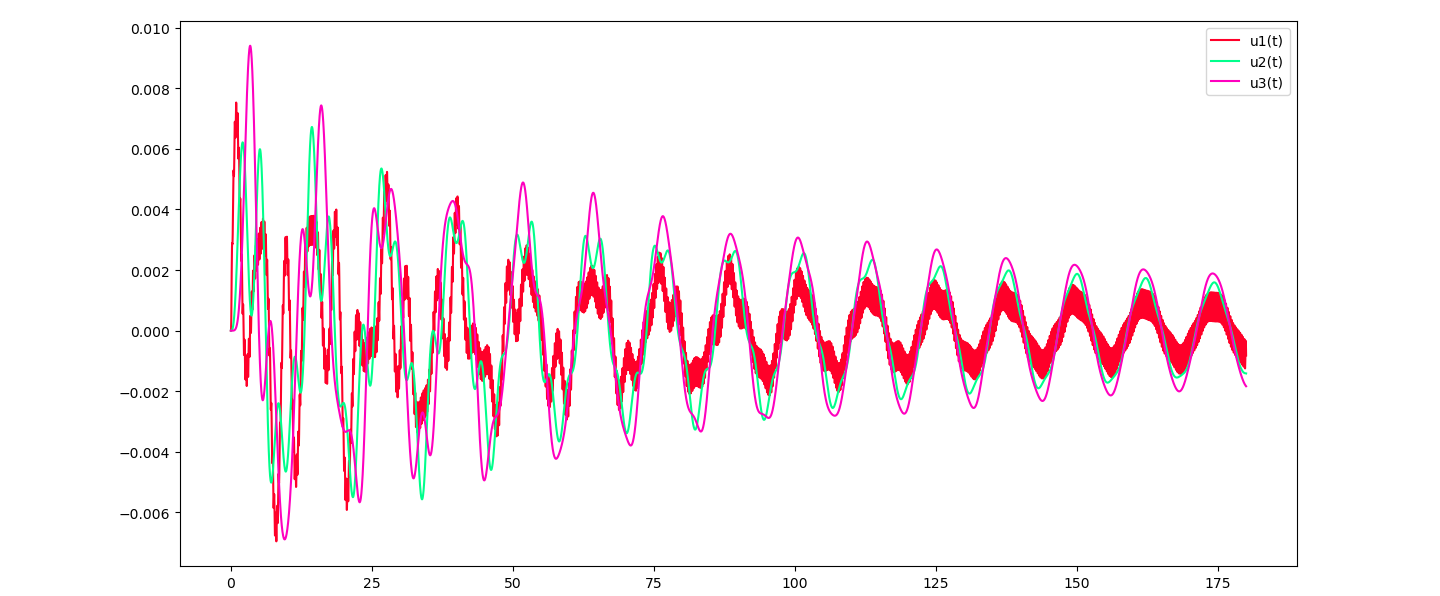
\includegraphics[width=\textwidth]{sol_sismo_largo}
    \caption{Gráfica de \(\mathbf{u}(t)\) con \(P_1(t) = m_1 A \sin(2\pi f t)\) para \(t \in [0, 180]\).}
    \label{fig:sol-sismo-largo}
\end{figure}

Si aumentamos las razones de amortiguamiento a
\[
    \zeta_1 = 10\%, \quad \zeta_2 = 5\%, \quad \zeta_3 = 2.5\%
,\]
se produce la figura~\ref{fig:sol-sismo-damped}. En esta gráfica, se puede notar que la amplitud de las vibraciones de la estructura se reduce más rápidamente que en la figura~\ref{fig:sol-sismo-largo}.

\begin{figure}[ht!]
    \centering
    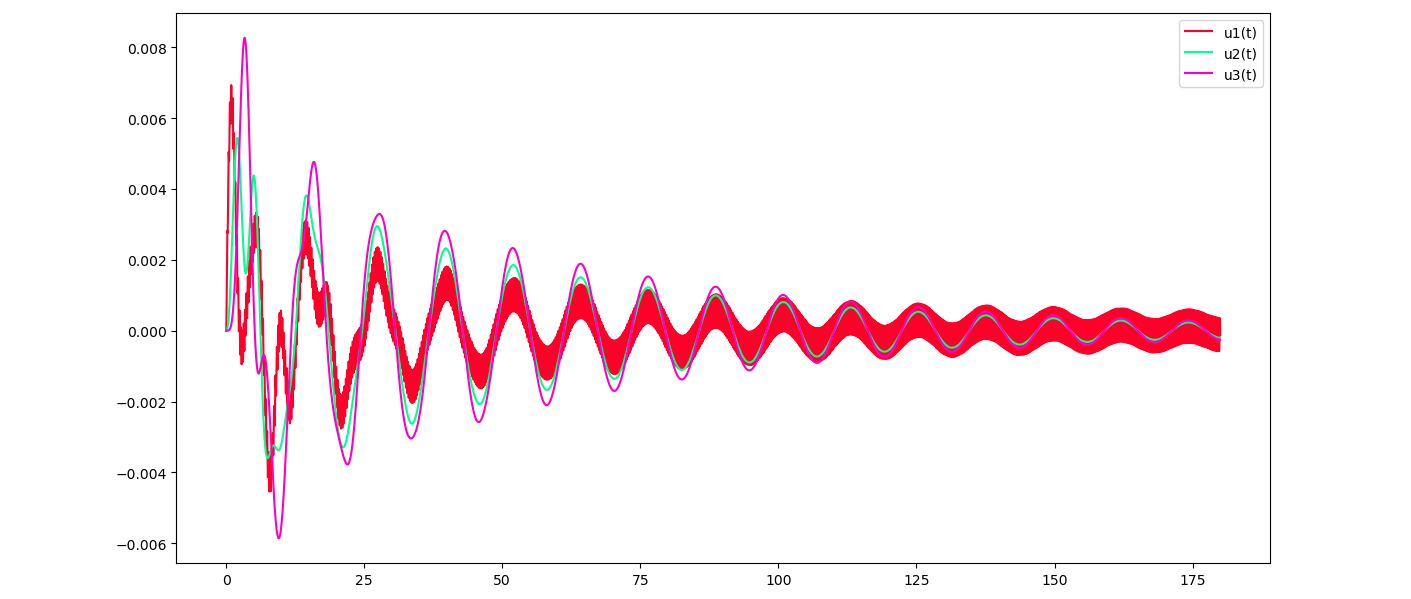
\includegraphics[width=\textwidth]{sol_sismo_damped}
    \caption{Gráfica de \(\mathbf{u}(t)\) con \(P_1(t) = m_1 A \sin(2\pi f t)\) para \(t \in [0, 180]\) (amortiguamiento aumentado).}
    \label{fig:sol-sismo-damped}
\end{figure}

Si, en lugar de aumentar el amortiguamiento, aumentamos los coeficientes elásticos a
\[
    k_1 = 200,000 \, \si{N/m}, \quad k_2 = 500,000 \, \si{N/m}, \quad k_3 = 800,000 \, \si{N/m}
,\]
se obtiene la figura~\ref{fig:sol-sismo-elastic}.

\begin{figure}[ht!]
    \centering
    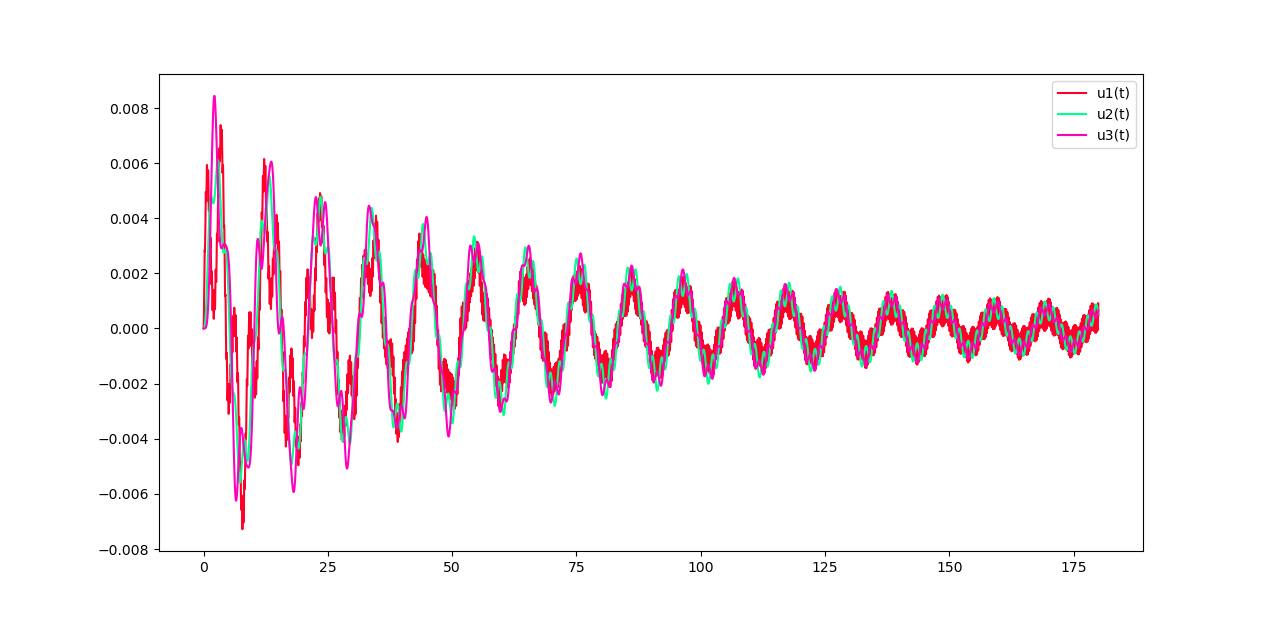
\includegraphics[width=\textwidth]{sol_sismo_elastic}
    \caption{Gráfica de \(\mathbf{u}(t)\) con \(P_1(t) = m_1 A \sin(2\pi f t)\) para \(t \in [0, 180]\) (elasticidad aumentada).}
    \label{fig:sol-sismo-elastic}
\end{figure}
